\section{Image (b)}

\noindent
\begin{minipage}[t]{0.49\textwidth}

    For \cref{fig:graph-b}, we have nodes $\hyperlink{fig:graph-b:v1}{v_1}$, $\hyperlink{fig:graph-b:v2}{v_2}$, $\hyperlink{fig:graph-b:v3}{v_3}$ and $\hyperlink{fig:graph-b:v4}{v_4}$ with degree odd ($\deg(v_i) = 3$ for $i = \hyperlink{fig:graph-b:v1}{1}$, $\hyperlink{fig:graph-b:v2}{2}$, $\hyperlink{fig:graph-b:v3}{3}$ and $\hyperlink{fig:graph-b:v4}{4}$), therefore the graph does \textbf{not} have an Euler trail and cannot be drawn without raising the pencil or repeating a line.

\end{minipage}%
\begin{minipage}[t]{0.5\textwidth}

    \begin{figure}[H]
        \centering
        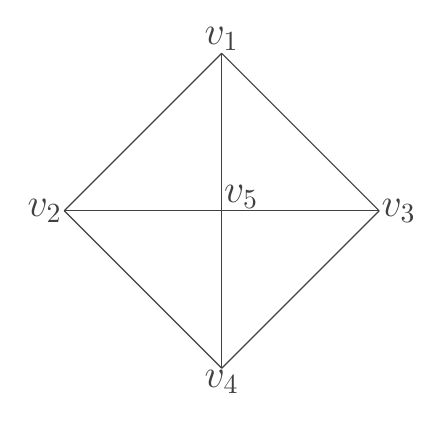
\begin{tikzpicture}[draw=darkgray, text=darkgray, align=center, node distance=2cm]
    \tikzstyle{every node}=[inner sep=0pt];

    \node (v5) [label=above right:{\Large $v_5$}] {};
    \node (v1) [label=above:{\Large $v_1$}, above of = v5] {};
    \node (v2) [label=left:{\Large $v_2$}, left of = v5] {};
    \node (v3) [label=right:{\Large $v_3$}, right of = v5] {};
    \node (v4) [label=below:{\Large $v_4$}, below of = v5] {};

    \path (v1.center)
        edge (v2.center)
        edge (v3.center);
    \path (v4.center)
        edge (v2.center)
        edge (v3.center);
    \path (v5.center)
        edge (v1.center)
        edge (v2.center)
        edge (v3.center)
        edge (v4.center);
\end{tikzpicture}


        \caption{Image \texttt{b.} with labelled nodes.}
        \label{fig:graph-b}
    \end{figure}

\end{minipage}
